\documentclass[aspectratio=169, 10pt]{beamer}
\usepackage{graphicx} % Required for inserting images
\usepackage{booktabs}

\usetheme{Boadilla}
%\usefonttheme{serif}

\usepackage{tikz}
\setbeamertemplate{background}{
  \begin{tikzpicture}[remember picture,overlay]
    \node[anchor=north east, xshift=-5mm, yshift=-3.5mm] at (current page.north east) {
      
\includegraphics[height=.75cm]{pics/WHU_Logo_RGB_Screen.jpg}
    };
  \end{tikzpicture}
}

\usecolortheme[]{dolphin}
\definecolor{WHUblue}{rgb}{.08, .27,.58} % WHU Blue 
\setbeamercolor{structure}{fg=WHUblue}

\setbeamertemplate{itemize item}{\color{WHUblue}$\bullet$}
\setbeamertemplate{itemize subitem}{\color{WHUblue}$\circ$}
\setbeamertemplate{itemize subsubitem}{\color{WHUblue}$\cdot$}

\setbeamercolor{block title}{bg=WHUblue!10, fg=WHUblue}
\setbeamercolor{block body}{bg=WHUblue!5, fg=black}
\setbeamertemplate{blocks}[default]  % ohne Schatten

\setbeamercolor{quoteblock title}{fg=WHUblue}
\setbeamercolor{quoteblock body}{bg=WHUblue!5}

\newenvironment{quoteblock}[1]{%
  \begin{beamercolorbox}[colsep*=.75ex, leftskip=1em, rightskip=1em, width=\textwidth, rounded=true]{quoteblock body}
  \textit{#1}
  \end{beamercolorbox}
}{}


\setbeamersize{text margin left=0.75cm, text margin right=0.75cm}

\setbeamertemplate{navigation symbols}{} % Symbole aus

\setbeamertemplate{headline}{%
  \leavevmode%
  \hspace{1em}%
  \usebeamercolor[fg]{section in head/foot}%
  \bfseries\insertsection%
  \vspace{0.5em}%
}

\newcommand{\source}[1]{%
  \tikz[remember picture,overlay]{
    \node[anchor=south east, xshift=-0.5cm, yshift=0.5cm] 
    at (current page.south east) {\scriptsize\color{gray!60}#1};
  }%
}

\newcommand{\twocolslide}[3]{%
  \begin{frame}
    \frametitle{#1}
    \begin{columns}[T,onlytextwidth]
      \begin{column}{0.65\textwidth}
        #2 % left side (usually text)
      \end{column}
      \begin{column}{0.4\textwidth}
        #3 % right side (usually image)
      \end{column}
    \end{columns}
  \end{frame}
}

\AtBeginSection[]{
  \begin{frame}[plain]
    \centering
    {\color{WHUblue}\LARGE\bfseries\insertsection}
  \end{frame}
}

\AtBeginSubsection[]{
  \begin{frame}[plain]
    \centering
    \vfill
    {\color{WHUblue}\large\insertsection}
    
    \vspace{1em}
    \color{WHUblue}\Huge\bfseries\insertsubsection
    \vfill
  \end{frame}
}

\title{Business Ethics}
\subtitle{Bachelor of Business Administration WHU}
\author[Rilke]{Prof. Rainer Michael Rilke }
\date{2025}

\begin{document}

\maketitle
\section{Introduction}

\begin{frame}
\frametitle{Moral}

\begin{itemize}
    \item oral lt. moralis: concerning custom; mos, mores: custom, customs
    \item Moral can be understood as a system of norms
    \item These norms relate to human behavior
    \item They have a certain unconditional claim to validity
\end{itemize}

\begin{itemize}
    \item Moral = morally good
    \item Immoral = morally evil, wrong, bad
\end{itemize}

\begin{itemize}
    \item Distinguish between:
    \item Norms of a moral
    \item Social norms
    \item Legal norms
\end{itemize}

\source{Reference: Hübner (2014)}
\end{frame}

% Slide 4
\begin{frame}
\frametitle{Example: Descriptive Ethics}

\begin{quote}
    "How selfish soever man may be supposed, there are evidently some principles in his nature, which interest him in the fortune of others, and render their happiness necessary to him, though he derives nothing from it except the pleasure of seeing it. Of this kind is pity or compassion, the emotion which we feel for the misery of others, when we either see it, or are made to conceive it in a very lively manner. That we often derive sorrow from the sorrow of others, is a matter of fact too obvious to require any instances to prove it; for this sentiment, like all the other original passions of human nature, is by no means confined to the virtuous and humane, though they perhaps may feel it with the most exquisite sensibility. The greatest ruffian, the most hardened violator of the laws of society, is not altogether without it." --- Adam Smith (1723-1790)
\end{quote}

\end{frame}

\begin{frame}{Test}

\begin{block}{Definition: Moral}
A system of norms relating to human behavior, claiming universal validity.
\end{block}
    
\end{frame}

\twocolslide{Title}{
here comes the textr
}
{
\includegraphics[height=3cm]{pics/WHU_Logo_RGB_Screen.jpg}
}


\subsection{Introduction to Business Ethics}
\subsection{Procedural Details}
\twocolslide{About me}{

\textbf{Education}
\begin{itemize}
  \item University Bonn (Dipl.)
  \item University of Cologne (PhD)
  \item Joined WHU in 2016
  \item Full Professor of Behavioral Economics since 2025
\end{itemize}
\textbf{Teaching Experience}
\begin{itemize}
  \item Bachelor, Master, and MBA level
\end{itemize}

\textbf{Research Interest}
\begin{itemize}
  \item Behavioral and Experimental Economics
  \item Interaction of Humans and Machines (AI)
  \item Incentives and Ethical Behavior
\end{itemize}

}{
\centering
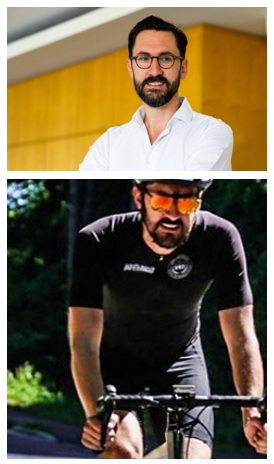
\includegraphics[height=6cm]{pics/rilke.PNG}
}

\begin{frame}
\frametitle{Course Schedule}
\centering
\begin{tabular}{@{}lcp{8cm}@{}}
\toprule
\textbf{Date} & \textbf{Session} & \textbf{Topic} \\
\midrule
Sep 5   & 1 & Introduction to Business Ethics \\
Sep 12  & 2 & Ethical Theories and Frameworks \\
Sep 19  & 3 & Behavioral Ethics: Why Good People Do Bad Things \\
Sep 26  & 4 & Ethics in Corporate Decision-Making \\
Oct 3   & 5 & Fairness, Justice, and Moral Intuition \\
Oct 10  & 6 & Case Study Discussion and Wrap-Up \\
\midrule
Oct 17  & &\textbf{Final Exam} \\
\bottomrule
\end{tabular}
\end{frame}

\begin{frame}{Lecture Materials}

\begin{itemize}
  \item All materials (slides, readings, cases, and additional resources) are available on the course GitHub repository:
  
  \vspace{0.5em}
  \begin{center}
      \texttt{\href{https://github.com/rrilke/BusinessEthics-WHU}{github.com/rrilke/BusinessEthics-WHU}}
  \end{center}
  \vspace{0.5em}

  \item Please check the repository regularly — it is the central source for everything.
  
  \item \textbf{Readings are essential:}
  \begin{itemize}
    \item \textbf{Required readings} must be read \emph{before class}.
    \item They are fundamental to understanding the course content and performing well in the final exam.
  \end{itemize}
  \item \textbf{Optional readings} are for those who want to dig deeper — or outperform everyone else. 
  \item I expect thoughtful and active engagement with the texts. They are not decorative.
\end{itemize}

\end{frame}
 
\begin{frame}
\frametitle{Final Exam}

\begin{itemize}
  \item \textbf{Duration:} 90 minutes
  \item \textbf{Total points:} 100
  \item \textbf{Format:}
  \begin{itemize}
    \item Multiple-choice questions
    \item Case study-based analysis
    \item Open-ended questions on key concepts discussed in class
  \end{itemize}
  \item \textbf{Scope:} All lecture content and required readings
  \item \textbf{Grading:} According to the official WHU grading scale
  \item \textbf{Focus:} Apply what you’ve learned — not just reproduce it
  \begin{itemize}
    \item You will be asked to transfer concepts to unfamiliar, real-world scenarios
  \end{itemize}
\end{itemize}

\vspace{0.8em}
\centering
\textit{Tip: Understanding and flexible thinking matter more than memorization.}
\end{frame}

\begin{frame}
\frametitle{ChatGPT Exam Question Challenge}

\begin{itemize}
  \item \textbf{Optional bonus assignment:} earn up to \textbf{10 extra points}
  \item Submit \textbf{5 self-generated exam-style questions} created using ChatGPT
  \begin{itemize}
    \item Varying difficulty: at least one basic, others more advanced
    \item Include different course topics and formats (MC or open-ended)
    \item Each question must include a \textbf{model answer}
  \end{itemize}
  \item Submit detailed documentation for each question:
  \begin{itemize}
    \item Prompt(s) used with ChatGPT
    \item ChatGPT’s raw output
    \item Short reflection on the process (2–4 sentences)
  \end{itemize}
  \item \textbf{Format:} PDF or Markdown file, named \texttt{Lastname\_Firstname\_BonusQuestions.pdf}
  \item \textbf{Deadline:} \textit{[Insert Date]}
\end{itemize}

\vspace{0.8em}
\centering
\textit{A chance to deepen your understanding and critically explore generative AI in learning.}
\end{frame}


\section{Ethical Theories}

\subsection{Utilitarianism}
\subsection{Deontology}
\subsection{Virtue Ethics}

\section{Behavioral Ethics}

\section{Corporate Responsibility \& Sustainability}
\section{Marketing, Accounting \& Transparency}
\section{Finance, Incentives \& Corruption}

\end{document}